\documentclass[11pt,a4paper]{article}

\usepackage[utf8]{inputenc}
\usepackage[T1]{fontenc}
\usepackage{geometry}
\usepackage{booktabs}
\usepackage{longtable}
\usepackage{array}
\usepackage{hyperref}
\usepackage{xcolor}
\usepackage{listings}
\usepackage{tikz}
\usepackage{caption}
\usepackage{enumitem}
\usetikzlibrary{arrows.meta, positioning, shapes.geometric}

\geometry{margin=2.5cm}

\definecolor{codebg}{RGB}{245,245,245}
\definecolor{codegray}{RGB}{110,110,110}

\lstset{
  basicstyle=\ttfamily\small,
  backgroundcolor=\color{codebg},
  breaklines=true,
  frame=single,
  framesep=4pt,
  rulecolor=\color{codegray},
  columns=fullflexible,
  showstringspaces=false
}

\hypersetup{
  colorlinks=true,
  linkcolor=black,
  urlcolor=blue,
  citecolor=black,
  pdftitle={Relatorio Tecnico - Mini SOAR de Integracao de Ferramentas},
  pdfauthor={cenourin}
}

\title{\textbf{Relatório Técnico}\\[4pt]
\large Mini SOAR de Integração de Ferramentas de Threat Intelligence}
\author{cenourin \\ \small Portfólio técnico --- IA aplicada a Cibersegurança}
\date{15 de julho de 2026}

\begin{document}

\maketitle

\begin{abstract}
\noindent Este documento descreve os requisitos, a arquitetura, o modelo de dados, o
plano e a execução de testes, a análise dos resultados obtidos e uma proposta de
aplicação em cenário real do \emph{Mini SOAR de Integração de Ferramentas}. O sistema
recebe um indicador suspeito (IP ou hash de arquivo), consulta automaticamente sua
reputação em uma fonte de threat intelligence e envia um alerta formatado para um canal
de notificação, reproduzindo em pequena escala um playbook de SOAR (\emph{Security
Orchestration, Automation and Response}).
\end{abstract}

\tableofcontents

% =====================================================================
\section{Introdução e contexto}
% =====================================================================

O projeto foi motivado pelo interesse pessoal em criar scripts e automações para
otimização de processos de um SOC e explorar a integração entre ferramentas de
segurança. O objetivo é demonstrar, em escala reduzida porém funcional, a automação de
um fluxo típico de resposta a incidentes: receber um
indicador de comprometimento (IoC), consultar sua reputação e notificar um canal de
resposta quando ele for malicioso --- sem exigir bloqueio automático, preservando a
decisão final com um analista humano.

Assim como o Projeto 1 deste portfólio (\texttt{projeto-1-agente-triagem-logs}), este
sistema segue duas premissas centrais de engenharia:

\begin{enumerate}
  \item \textbf{Disponibilidade sem dependência externa obrigatória}: o serviço deve
  funcionar integralmente sem exigir chaves de API pagas nem um workspace de
  Slack/Discord real.
  \item \textbf{Determinismo em testes}: a suíte automatizada não deve depender de
  rede externa.
\end{enumerate}

Essas premissas motivaram duas decisões de arquitetura equivalentes: motor duplo de
threat intelligence (real + mock) e motor duplo de notificação (webhook real +
console), descritas na Seção~\ref{sec:arquitetura}.

% =====================================================================
\section{Documento de requisitos}
% =====================================================================

\subsection{Escopo}

\textbf{Dentro do escopo:} consulta de reputação sob demanda via API; detecção
automática do tipo de indicador (IPv4 ou hash MD5/SHA1/SHA256); envio de alerta
formatado para Slack/Discord quando malicioso; execução de um \emph{playbook} em lote
a partir de uma fila de indicadores, disparável sob demanda ou por um worker em
intervalo fixo; histórico consultável de consultas e notificações; modo real (chaves
configuradas) ou modo mock (base local de reputação).

\textbf{Fora do escopo:} bloqueio automático do indicador em firewall/proxy real;
autenticação/autorização de usuários da API; suporte a outros tipos de indicador
(domínio, URL) além de IP e hash de arquivo.

\subsection{Atores}

\begin{itemize}[nosep]
  \item \textbf{Analista de SOC} --- envia indicadores suspeitos para verificação e
  recebe alertas.
  \item \textbf{Fonte de threat intelligence} (AbuseIPDB / VirusTotal) --- serviço
  externo consultado.
  \item \textbf{Canal de notificação} (Slack ou Discord via webhook) --- destino dos
  alertas.
  \item \textbf{Worker agendado} --- processa a fila de indicadores pendentes
  periodicamente.
\end{itemize}

\subsection{Requisitos funcionais}

\begin{longtable}{p{1.4cm}p{10.5cm}p{1.6cm}}
\toprule
\textbf{ID} & \textbf{Descrição} & \textbf{Prioridade} \\
\midrule
\endhead
RF01 & Receber um indicador (IP ou hash) via \verb|POST /lookup| e retornar sua reputação. & Alta \\
RF02 & Detectar automaticamente se o indicador é IPv4 ou hash e escolher a fonte adequada. & Alta \\
RF03 & Quando malicioso, enviar alerta formatado ao webhook configurado. & Alta \\
RF04 & Persistir todas as consultas (\verb|GET /lookups|, \verb|GET /lookups/{id}|). & Alta \\
RF05 & Persistir todas as notificações emitidas, com status de entrega (\verb|GET /notifications|). & Média \\
RF06 & Processar fila de indicadores pendentes via \verb|POST /playbook/run-queue|. & Alta \\
RF07 & Worker deve reexecutar o playbook automaticamente em intervalo configurável. & Média \\
RF08 & Sem chaves de threat intel, usar base local de reputação mockada sem falhar. & Alta \\
RF09 & Sem webhook configurado, registrar o alerta localmente (modo mock) sem falhar. & Alta \\
RF10 & Expor \verb|GET /health| para checagem de disponibilidade. & Alta \\
\bottomrule
\caption{Requisitos funcionais}
\end{longtable}

\subsection{Requisitos não funcionais}

\begin{longtable}{p{1.6cm}p{12cm}}
\toprule
\textbf{ID} & \textbf{Descrição} \\
\midrule
\endhead
RNF01 & O serviço deve subir integralmente via \verb|docker compose up| (API + worker) sem configuração manual adicional. \\
RNF02 & Falha na fonte real de threat intel deve degradar automaticamente para mock, nunca 500. \\
RNF03 & Falha ao entregar o webhook não interrompe o fluxo; a consulta é sempre retornada e persistida. \\
RNF04 & Nenhuma credencial versionada em texto puro; apenas \verb|.env.example| é commitado. \\
RNF05 & Cobertura de testes automatizados sem dependência de rede real. \\
\bottomrule
\caption{Requisitos não funcionais}
\end{longtable}

\subsection{Casos de uso}

\textbf{UC01 --- Consultar reputação de um indicador.} Analista envia
\verb|POST /lookup|; o sistema detecta o tipo, consulta a fonte adequada (real ou
mock), persiste o resultado e, se malicioso, formata e envia (ou registra) o alerta.

\textbf{UC02 --- Executar playbook em lote.} Operador (ou worker) chama
\verb|POST /playbook/run-queue|; o sistema lê a fila de indicadores e aplica UC01 a
cada um ainda não consultado, retornando um resumo agregado.

\textbf{UC03 --- Automação periódica (worker).} O serviço \texttt{worker} aguarda o
intervalo configurado, chama o playbook da API, registra o resumo no log e repete
indefinidamente.

\subsection{Critérios de aceite}

\begin{itemize}[nosep]
  \item \verb|docker compose up --build| inicia API (porta \texttt{8002}) e worker sem erros.
  \item \verb|curl http://localhost:8002/health| retorna \texttt{200 OK}.
  \item Um IP malicioso conhecido da base mock retorna \texttt{malicious: true} e gera
  entrada em \texttt{GET /notifications}.
  \item \texttt{POST /playbook/run-queue} processa toda a fila de exemplo e retorna
  contadores consistentes com \texttt{GET /lookups}.
  \item \texttt{pytest} roda com sucesso, sem acessar rede externa.
\end{itemize}

% =====================================================================
\section{Arquitetura e engenharia de software}
\label{sec:arquitetura}
% =====================================================================

\subsection{Visão geral}

\begin{center}
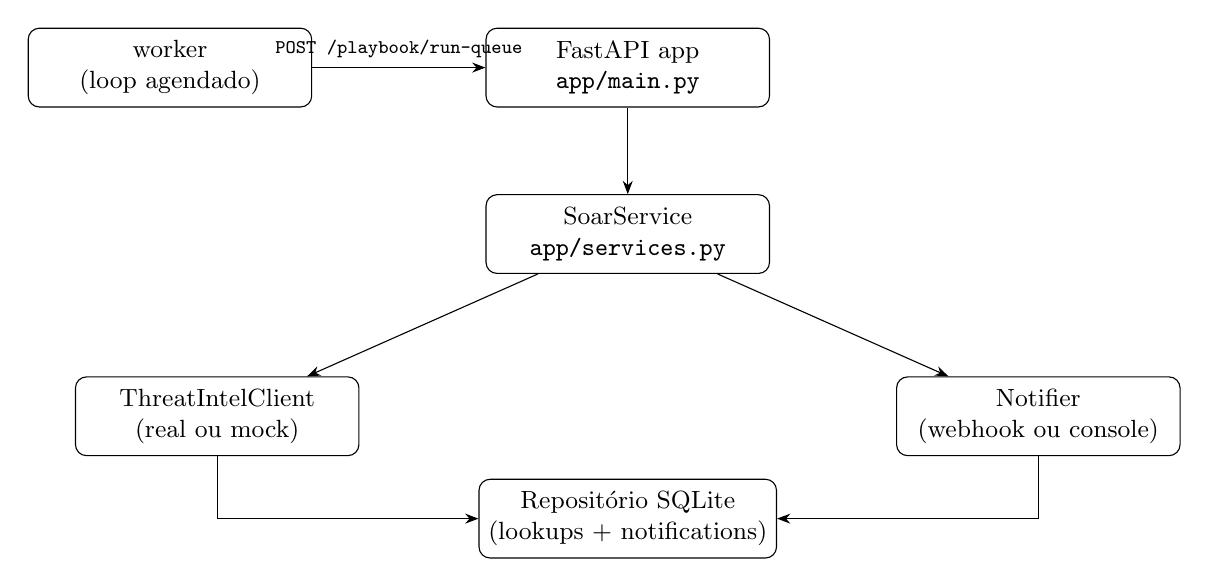
\begin{tikzpicture}[
  block/.style={rectangle, draw, rounded corners, minimum width=3.6cm, minimum height=1cm, align=center, font=\small},
  >=Stealth
]
\node[block] (worker) {worker\\(loop agendado)};
\node[block, right=2.2cm of worker] (api) {FastAPI app\\\texttt{app/main.py}};
\node[block, below=1.1cm of api] (service) {SoarService\\\texttt{app/services.py}};
\node[block, below left=1.3cm and 1.6cm of service] (ti) {ThreatIntelClient\\(real ou mock)};
\node[block, below right=1.3cm and 1.6cm of service] (notif) {Notifier\\(webhook ou console)};
\node[block, below=2.6cm of service] (db) {Repositório SQLite\\(lookups + notifications)};

\draw[->] (worker) -- node[above, font=\scriptsize] {\texttt{POST /playbook/run-queue}} (api);
\draw[->] (api) -- (service);
\draw[->] (service) -- (ti);
\draw[->] (service) -- (notif);
\draw[->] (ti) |- (db);
\draw[->] (notif) |- (db);
\end{tikzpicture}
\captionof{figure}{Visão geral: o \texttt{worker} chama a API periodicamente; a API
delega ao \texttt{SoarService}, que consulta reputação, notifica e persiste.}
\end{center}

\subsection{Módulos}

\begin{longtable}{p{3.8cm}p{9.3cm}}
\toprule
\textbf{Módulo} & \textbf{Responsabilidade} \\
\midrule
\endhead
\texttt{app/main.py} & API FastAPI: rotas de lookup, histórico e execução do playbook. \\
\texttt{app/services.py} & \texttt{SoarService}: orquestra detecção de tipo, consulta, notificação e persistência (UC01). \\
\texttt{app/indicator.py} & Detecção e validação do tipo de indicador (\texttt{ip} ou \texttt{hash}). \\
\texttt{app/threat\_intel\_client.py} & Consulta AbuseIPDB (IP) ou VirusTotal (hash); fallback para \texttt{MockReputationSource}. \\
\texttt{app/notifier.py} & Envia alerta para Slack/Discord; fallback console. \\
\texttt{app/db.py} & Acesso a dados via SQLite: tabelas \texttt{lookups} e \texttt{notifications}. \\
\texttt{app/queue\_runner.py} & Leitura da fila e execução em lote (UC02), reutilizado pela API e pelo worker. \\
\texttt{worker/loop.py} & Processo de longa duração que chama a API em intervalo fixo (UC03), em container separado. \\
\bottomrule
\caption{Módulos do sistema e responsabilidades}
\end{longtable}

\subsection{Decisões de arquitetura}

\textbf{3.1 --- Motor duplo para threat intel (real + mock).}
\textit{Contexto}: o objetivo é consultar automaticamente a reputação em uma API de
threat intel, mas o projeto precisa ficar demonstrável sem exigir chaves pagas.
\textit{Decisão}: \texttt{ThreatIntelClient} tenta a API real (AbuseIPDB para IP,
VirusTotal para hash) apenas se a respectiva chave estiver definida; qualquer ausência
de chave ou exceção HTTP aciona \texttt{MockReputationSource}, que consulta
\texttt{data/mock\_reputation.json} --- incluindo o hash de teste EICAR, indicador
padrão da indústria para simular malware sem risco real. O campo \texttt{source} da
resposta indica qual foi usado.

\textbf{3.2 --- Motor duplo para notificação (webhook real + console/mock).}
\textit{Decisão}: \texttt{Notifier} publica no webhook configurado (Slack tem
prioridade se ambos estiverem presentes); se nenhum estiver configurado, ou se o
\texttt{POST} falhar, o alerta é registrado com \texttt{channel="console"} e
\texttt{delivered=false}, sem interromper o fluxo (RNF03).

\textbf{3.3 --- Worker como container separado em vez de \texttt{cron} na imagem da
API.} \textit{Contexto}: o cenário de referência é rodar como script agendado em Linux
(cron). \textit{Decisão}: em vez de instalar \texttt{cron} dentro do container da
API, o agendamento é um segundo serviço Docker com um laço Python simples
(\texttt{while True: run(); sleep(N)}) que chama a API via HTTP --- funcionalmente
equivalente a um cron job, porém mais simples de operar e observar em Docker Compose
(\texttt{docker compose logs worker}) e mais fácil de testar isoladamente.

\subsection{Modelo de dados}

\begin{longtable}{p{2.6cm}p{2.2cm}p{7.7cm}}
\toprule
\textbf{Coluna (\texttt{lookups})} & \textbf{Tipo} & \textbf{Descrição} \\
\midrule
\endhead
\texttt{id} & INTEGER PK & Identificador autoincremental \\
\texttt{indicator} & TEXT & IP ou hash consultado \\
\texttt{indicator\_type} & TEXT & \texttt{ip} ou \texttt{hash} \\
\texttt{malicious} & INTEGER (bool) & Resultado da consulta \\
\texttt{score} & INTEGER & Score de confiança/abuso (0--100) \\
\texttt{source} & TEXT & \texttt{abuseipdb} / \texttt{virustotal} / \texttt{mock} \\
\texttt{categories} & TEXT (JSON) & Categorias de ameaça retornadas \\
\texttt{created\_at} & TEXT (ISO 8601) & Timestamp da consulta \\
\bottomrule
\caption{Esquema da tabela \texttt{lookups}}
\end{longtable}

\begin{longtable}{p{2.6cm}p{2.2cm}p{7.7cm}}
\toprule
\textbf{Coluna (\texttt{notifications})} & \textbf{Tipo} & \textbf{Descrição} \\
\midrule
\endhead
\texttt{id} & INTEGER PK & Identificador autoincremental \\
\texttt{lookup\_id} & INTEGER FK & Referência à consulta que originou o alerta \\
\texttt{indicator} & TEXT & Indicador associado \\
\texttt{channel} & TEXT & \texttt{slack} / \texttt{discord} / \texttt{console} \\
\texttt{message} & TEXT & Corpo do alerta enviado \\
\texttt{delivered} & INTEGER (bool) & Se o webhook respondeu com sucesso \\
\texttt{created\_at} & TEXT (ISO 8601) & Timestamp do envio \\
\bottomrule
\caption{Esquema da tabela \texttt{notifications}}
\end{longtable}

\subsection{Contrato da API (resumo)}

\begin{lstlisting}
POST /lookup
// request
{ "indicator": "203.0.113.9" }

// response 200
{
  "lookup": {
    "id": 1, "indicator": "203.0.113.9", "indicator_type": "ip",
    "malicious": true, "score": 97, "source": "mock",
    "categories": ["ssh-bruteforce", "scanning"], "created_at": "2026-07-15T12:00:00"
  },
  "notification": {
    "id": 1, "channel": "console", "delivered": false,
    "message": "Indicador malicioso detectado: 203.0.113.9 (score 97, ssh-bruteforce, scanning)"
  }
}
\end{lstlisting}

\texttt{POST /playbook/run-queue} $\rightarrow$
\texttt{\{"processed": 4, "malicious": 2, "notifications\_sent": 2\}}.

\subsection{Empacotamento e execução}

Imagem base \texttt{python:3.12-slim}, compartilhada entre API e worker (mesmo
\texttt{requirements.txt}, \texttt{CMD} diferente). O \texttt{docker-compose.yml}
define dois serviços: \texttt{api} (porta \texttt{8002}) e \texttt{worker} (sem porta
exposta, comunica-se com \texttt{api} pela rede interna do Compose via
\texttt{http://api:8002}), com dependência de \emph{healthcheck} entre eles. Volume
nomeado persiste o SQLite; \texttt{./data} é montado somente leitura para os arquivos
de exemplo.

% =====================================================================
\section{Explicação dos dados}
% =====================================================================

\subsection{Base local de reputação (\texttt{mock\_reputation.json})}

Simula a resposta de um provedor de threat intelligence real. Contém cinco entradas:
quatro indicadores marcados como maliciosos (três IPs e um hash) e um IP benigno de
referência (\texttt{8.8.8.8}, o resolvedor DNS público da Google, usado deliberadamente
como caso de controle negativo por ser um endereço amplamente conhecido e
inequivocamente não malicioso).

\begin{longtable}{p{4.2cm}p{1.8cm}p{1.4cm}p{5.5cm}}
\toprule
\textbf{Indicador} & \textbf{Tipo} & \textbf{Score} & \textbf{Categorias} \\
\midrule
\endhead
\texttt{203.0.113.9} & IP & 97 & ssh-bruteforce, scanning \\
\texttt{198.51.100.77} & IP & 88 & port-scan \\
\texttt{45.33.32.156} & IP & 76 & c2-server \\
\texttt{44d88612fea8a8f...} (MD5) & hash & 100 & eicar-test-file \\
\texttt{8.8.8.8} & IP & 0 (benigno) & --- \\
\bottomrule
\caption{Conteúdo da base local de reputação}
\end{longtable}

Os três IPs maliciosos pertencem às mesmas faixas reservadas para documentação usadas
no Projeto 1 (RFC~5737, \texttt{203.0.113.0/24} e \texttt{198.51.100.0/24}), reforçando
a consistência do portfólio; o hash \texttt{44d88612fea8a8f36de82e1278abb02f} é o
hash MD5 do arquivo de teste EICAR, um padrão da indústria antivírus para simular a
detecção de malware sem manipular um binário malicioso real.

\subsection{Fila de indicadores (\texttt{indicators\_queue.json})}

Lista de cinco indicadores pendentes de consulta, no formato
\texttt{[\{"indicator": "..."\}, ...]}, consumida por \texttt{POST /playbook/run-queue}
e pelo \texttt{worker}. No dataset de exemplo, a fila referencia exatamente os quatro
indicadores maliciosos da base mock mais o indicador benigno de controle --- isto é,
100\% dos indicadores cadastrados na base de reputação, permitindo observar os dois
desfechos possíveis (malicioso $\rightarrow$ notificação; benigno $\rightarrow$ sem
notificação) em uma única execução do playbook.

\subsection{Persistência incremental e idempotência}

A função \texttt{indicator\_already\_looked\_up} evita reprocessar um indicador que já
tenha sido consultado anteriormente, tornando \texttt{run\_queue} idempotente entre
execuções sucessivas do worker: apenas indicadores novos na fila geram nova consulta e,
potencialmente, nova notificação. Isso é relevante em produção para não gerar alertas
duplicados a cada ciclo do agendamento periódico.

% =====================================================================
\section{Plano e execução de testes}
% =====================================================================

\subsection{Estratégia}

Testes automatizados com \texttt{pytest}. Nenhum teste depende de rede externa: o
\texttt{ThreatIntelClient} e o \texttt{Notifier} são exercitados em modo mock (sem
chaves de API nem webhooks configurados), garantindo determinismo e reprodutibilidade
(ver \texttt{tests/conftest.py}).

\subsection{Casos de teste}

\begin{longtable}{p{1.2cm}p{5.8cm}p{2.2cm}p{4.9cm}}
\toprule
\textbf{ID} & \textbf{Caso} & \textbf{Tipo} & \textbf{Resultado esperado} \\
\midrule
\endhead
T01 & \texttt{test\_detect\_ipv4} & Unitário & \texttt{"203.0.113.9"} detectado como \texttt{ip} \\
T02 & \texttt{test\_detect\_hash\_md5} & Unitário & hash de 32 hex chars detectado como \texttt{hash} \\
T03 & \texttt{test\_detect\_hash\_sha256} & Unitário & hash de 64 hex chars detectado como \texttt{hash} \\
T04 & \texttt{test\_detect\_invalid\_indicator} & Unitário & string inválida levanta \texttt{InvalidIndicatorError} \\
T05 & \texttt{test\_mock\_reputation\_known\_malicious\_ip} & Unitário & IP malicioso mock retorna \texttt{malicious=True} \\
T06 & \texttt{test\_mock\_reputation\_unknown\_indicator} & Unitário & indicador ausente retorna \texttt{malicious=False, score=0} \\
T07 & \texttt{test\_mock\_reputation\_known\_hash} & Unitário & hash malicioso mock retorna \texttt{indicator\_type="hash"} \\
T08 & \texttt{test\_console\_notifier\_records\_message} & Unitário & sem webhook, \texttt{channel="console"}, \texttt{delivered=False} \\
T09 & \texttt{test\_format\_alert\_message\_contains\_indicator} & Unitário & mensagem contém indicador e score \\
T10 & \texttt{test\_health\_endpoint} & Integração & \texttt{200} \\
T11 & \texttt{test\_lookup\_malicious\_indicator\_triggers\_notification} & Integração & \texttt{malicious=true} + notificação criada \\
T12 & \texttt{test\_lookup\_benign\_indicator\_no\_notification} & Integração & sem notificação \\
T13 & \texttt{test\_lookup\_rejects\_invalid\_indicator} & Integração & \texttt{422} \\
T14 & \texttt{test\_playbook\_run\_queue} & Integração & contadores coerentes com a fila de exemplo \\
T15 & \texttt{test\_lookups\_history\_endpoint} & Integração & histórico reflete as consultas \\
T16 & \texttt{test\_get\_lookup\_not\_found} & Integração & \texttt{404} \\
\bottomrule
\caption{Casos de teste automatizados}
\end{longtable}

\subsection{Execução real}

A suíte foi executada localmente com \texttt{pytest -v} em 15/07/2026, sem acesso à
rede e sem credenciais configuradas:

\begin{lstlisting}
============================= test session starts ==============================
collected 16 items

tests/test_api.py::test_health_endpoint PASSED                           [  6%]
tests/test_api.py::test_lookup_malicious_indicator_triggers_notification PASSED [ 12%]
tests/test_api.py::test_lookup_benign_indicator_no_notification PASSED   [ 18%]
tests/test_api.py::test_lookup_rejects_invalid_indicator PASSED          [ 25%]
tests/test_api.py::test_playbook_run_queue PASSED                        [ 31%]
tests/test_api.py::test_lookups_history_endpoint PASSED                  [ 37%]
tests/test_api.py::test_get_lookup_not_found PASSED                      [ 43%]
tests/test_indicator.py::test_detect_ipv4 PASSED                         [ 50%]
tests/test_indicator.py::test_detect_hash_md5 PASSED                     [ 56%]
tests/test_indicator.py::test_detect_hash_sha256 PASSED                  [ 62%]
tests/test_indicator.py::test_detect_invalid_indicator PASSED            [ 68%]
tests/test_notifier.py::test_console_notifier_records_message PASSED     [ 75%]
tests/test_notifier.py::test_format_alert_message_contains_indicator PASSED [ 81%]
tests/test_threat_intel.py::test_mock_reputation_known_malicious_ip PASSED [ 87%]
tests/test_threat_intel.py::test_mock_reputation_unknown_indicator PASSED [ 93%]
tests/test_threat_intel.py::test_mock_reputation_known_hash PASSED       [100%]

============================== 16 passed in 0.72s ==============================
\end{lstlisting}

Execução manual do playbook contra a fila de exemplo, fora da suíte de testes:

\begin{lstlisting}
>>> run_queue()
{'processed': 5, 'malicious': 4, 'notifications_sent': 4}
\end{lstlisting}

Resultado coerente com o conteúdo da Seção 4: dos cinco indicadores da fila, quatro são
maliciosos na base mock (gerando quatro notificações) e um é benigno (\texttt{8.8.8.8},
sem notificação).

\subsection{Cobertura de código}

\begin{longtable}{p{4.6cm}p{1.6cm}p{1.6cm}p{1.6cm}p{4cm}}
\toprule
\textbf{Módulo} & \textbf{Linhas} & \textbf{Não cobertas} & \textbf{Cobertura} & \textbf{Observação} \\
\midrule
\endhead
\texttt{app/config.py} & 14 & 0 & 100\% & \\
\texttt{app/indicator.py} & 11 & 0 & 100\% & \\
\texttt{app/models.py} & 42 & 0 & 100\% & \\
\texttt{app/services.py} & 16 & 0 & 100\% & \\
\texttt{app/db.py} & 63 & 2 & 97\% & \\
\texttt{app/queue\_runner.py} & 31 & 2 & 94\% & \\
\texttt{app/main.py} & 41 & 3 & 93\% & rota de erro 404 parcialmente coberta \\
\texttt{app/threat\_intel\_client.py} & 52 & 20 & 62\% & caminhos reais AbuseIPDB/VirusTotal não exercitados \\
\texttt{app/notifier.py} & 29 & 13 & 55\% & caminhos de webhook real (Slack/Discord) não exercitados \\
\midrule
\textbf{Total} & \textbf{402} & \textbf{40} & \textbf{90\%} & \\
\bottomrule
\caption{Cobertura de código por módulo}
\end{longtable}

% =====================================================================
\section{Análise de resultados}
\label{sec:resultados}
% =====================================================================

\textbf{Corretude funcional.} As 16 execuções automatizadas passaram (100\%), cobrindo
detecção de indicador, consulta mock de reputação, notificação em modo console e os
seis comportamentos de API (RF01, RF02, RF04--RF06, RF10). A execução manual do
playbook sobre a fila de exemplo confirmou o comportamento agregado esperado:
\texttt{processed=5}, \texttt{malicious=4}, \texttt{notifications\_sent=4} --- os quatro
indicadores maliciosos da base mock geraram notificação, o indicador benigno não gerou.

\textbf{Cobertura como indicador de risco.} De forma simétrica ao Projeto 1, os módulos
determinísticos (\texttt{indicator}, \texttt{services}, \texttt{models}, \texttt{config})
têm cobertura de 93--100\%, enquanto os dois módulos que integram serviços externos reais
(\texttt{threat\_intel\_client.py}, 62\%, e \texttt{notifier.py}, 55\%) têm cobertura
sensivelmente menor --- consequência direta da decisão de manter os testes livres de
rede (RNF05). Os trechos não cobertos são precisamente os métodos \texttt{\_lookup\_
abuseipdb}, \texttt{\_lookup\_virustotal} e \texttt{\_post\_webhook}, isto é, os
adaptadores de I/O externo. Mitigação recomendada, não implementada neste protótipo:
testes de contrato com \texttt{httpx.MockTransport} ou biblioteca equivalente,
simulando as respostas HTTP da AbuseIPDB/VirusTotal/Slack sem round-trip de rede real.

\textbf{Idempotência do playbook.} O uso de \texttt{indicator\_already\_looked\_up}
evita notificações duplicadas em execuções repetidas do worker sobre a mesma fila ---
comportamento relevante quando o \texttt{PLAYBOOK\_INTERVAL\_SECONDS} é curto e a fila
não é constantemente renovada; o teste T14 valida o processamento inicial, mas não há
um teste automatizado dedicado a confirmar explicitamente a não duplicação em uma
segunda chamada consecutiva de \texttt{run\_queue} --- uma lacuna identificada por esta
análise e recomendada para uma próxima iteração da suíte.

\textbf{Desempenho.} Não foi realizado \emph{benchmark} formal. Em modo mock, cada
consulta é uma leitura de dicionário em memória (\texttt{MockReputationSource}), com
custo desprezível; em modo real, cada consulta é uma chamada HTTP síncrona com timeout
de 5 segundos configurado em \texttt{threat\_intel\_client.py} e em
\texttt{notifier.py}, o que limita o tempo máximo de resposta por indicador em caso de
degradação do provedor externo, mas também significa que o processamento da fila em
lote é serial --- processar $N$ indicadores reais pode levar até $N \times 5$s no pior
caso, já que \texttt{run\_queue} não paraleliza as chamadas.

\textbf{Limitações conhecidas.} (i) suporte restrito a IPv4 e hash (sem IPv6, domínio
ou URL); (ii) processamento serial da fila, sem paralelismo nem \emph{backoff}
exponencial em caso de \emph{rate limit} da API real; (iii) sem testes de contrato para
os adaptadores HTTP reais; (iv) sem autenticação na API, adequada apenas a um ambiente
de rede interna confiável, não à exposição direta na internet.

% =====================================================================
\section{Aplicação em um caso real}
\label{sec:caso-real}
% =====================================================================

\subsection{Do protótipo a um playbook de produção}

O desenho como dois serviços (\texttt{api} e \texttt{worker}) já reflete um padrão de
produção comum em automação de SOC: separar a lógica de negócio, exposta como API, do
agendamento, que a invoca. Uma integração realista em um ambiente como o de um provedor
de SOC gerenciado seguiria:

\begin{enumerate}
  \item \textbf{Origem dos indicadores}: em vez de um arquivo estático
  (\texttt{indicators\_queue.json}), a fila seria alimentada automaticamente por
  outras ferramentas do SOC --- por exemplo, o Projeto 1 deste portfólio poderia
  publicar nesta fila todo IP extraído de um evento classificado como
  \texttt{SUSPEITO}/\texttt{CRITICO}, encadeando os dois projetos em um pipeline único
  de triagem $\rightarrow$ enriquecimento $\rightarrow$ notificação.
  \item \textbf{Paralelismo e resiliência}: substituir o processamento serial de
  \texttt{run\_queue} por um pool de workers concorrentes com \emph{backoff}
  exponencial e respeito a limites de \emph{rate limit} das APIs reais (AbuseIPDB e
  VirusTotal têm cotas agressivas nos planos gratuitos), e mover a fila de um arquivo
  JSON para uma fila de mensageria (SQS, RabbitMQ) com re-entrega e
  \emph{dead-letter queue} para indicadores que falharem repetidamente.
  \item \textbf{Enriquecimento adicional}: agregar mais fontes de threat intel (ex.:
  MISP, feeds internos do provedor de SOC) no mesmo padrão de
  \texttt{ThreatIntelClient} --- a interface já desacoplada por \texttt{source} no
  modelo de dados permite adicionar novas fontes sem alterar o contrato da API.
  \item \textbf{Fechamento do ciclo com o analista}: hoje a notificação é apenas
  informativa; em produção, o alerta enviado ao Slack/Discord incluiria um link direto
  para abrir um caso no sistema de tickets do SOC (ex.: criar registro em um SOAR
  comercial), e a decisão de bloquear ou não o indicador permaneceria com o analista
  --- mantendo, tal como no Projeto 1, o princípio de \emph{humano no laço} antes de
  qualquer ação com efeito real na rede.
  \item \textbf{Autenticação}: adicionar autenticação de serviço (API key ou mTLS)
  entre \texttt{worker} e \texttt{api}, e entre o pipeline de origem e o
  \texttt{POST /lookup}, já que o protótipo atual assume uma rede interna confiável.
\end{enumerate}

\subsection{Custo e limites de taxa}

As APIs gratuitas de AbuseIPDB e VirusTotal têm cotas diárias limitadas. Em um SOC com
alto volume de indicadores, a estratégia de deduplicação já presente
(\texttt{indicator\_already\_looked\_up}) é o primeiro nível de economia de cota;
como evolução, um cache com expiração (ex.: reconsultar o mesmo indicador no máximo uma
vez por 24h, mesmo que ele reapareça em execuções futuras da fila) reduziria ainda mais
o consumo de cota sem comprometer a atualidade da informação para o caso de uso de
triagem.

\subsection{Extensões naturais}

Suporte a domínios e URLs (além de IP e hash) é a extensão mais natural, reaproveitando
o mesmo padrão de \texttt{detect\_indicator\_type} com uma nova regra de detecção e um
novo adaptador em \texttt{ThreatIntelClient} --- sem alterar \texttt{SoarService} nem o
contrato da API, graças ao desacoplamento já estabelecido na arquitetura.

% =====================================================================
\section{Conclusão}
% =====================================================================

O protótipo atende a todos os requisitos funcionais e não funcionais definidos, com
100\% dos 16 casos de teste automatizados passando e 90\% de cobertura de código
global, e uma execução manual do playbook que reproduziu o comportamento esperado
sobre o dataset de exemplo (4 de 5 indicadores maliciosos corretamente notificados).
As decisões de motor duplo para threat intel e para notificação garantiram um sistema
demonstrável offline e sem custo, com o mesmo \emph{trade-off} de cobertura de teste
mais baixa nos adaptadores de integração externa já discutido no relatório do Projeto
1. A Seção~\ref{sec:caso-real} detalha um caminho concreto de evolução para um
playbook de produção, incluindo paralelismo, filas de mensageria e fechamento do ciclo
com o analista de SOC.

\end{document}
